%============================================================
\section{Nombre: Circulo protector.} \label{hab.CirPro}
\subsection{Descripción}
El enemigo se rodea a sí mismo con un circulo de tonalli corrupto. El circulo reducirá la cantidad de vida del jugador al hacer contacto con éste. El fuego no afectara a otros objetos que no sean el jugador. Mientras esta habilidad se encuentre activa, el enemigo no recibirá daño por parte del jugador. La única manera de desactivar esta habilidad es que el jugador destruya el circulo protector disparando tonalli de manera constante. 
\subsection{Portador}
Tlazoltéotl (ver apartado \ref{per:tlazolteotl}).
\subsection{Esquema}
			Ver figura \ref{fig:circuloP}.
			\begin{figure}
				\centering
				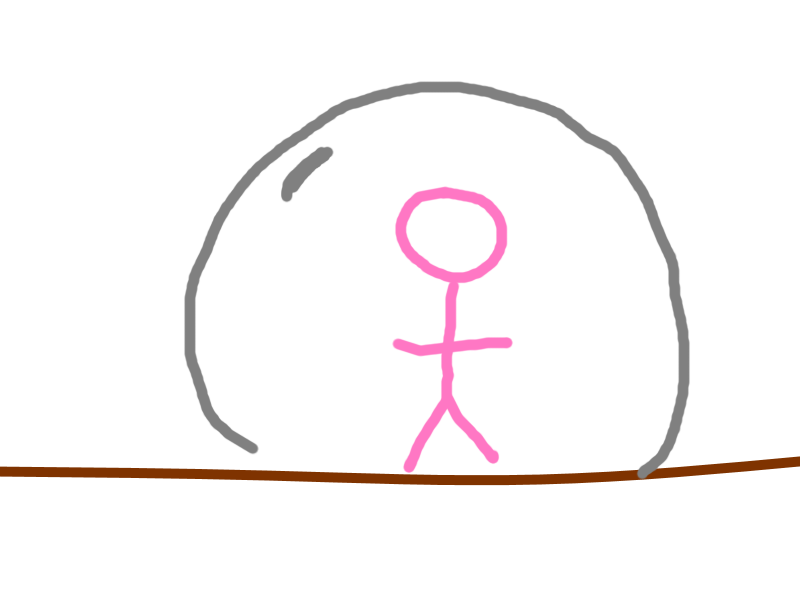
\includegraphics[height=0.2 \textheight]{Imagenes/circuloP}
				\caption{Círculo protector.}
				\label{fig:circuloP}
			\end{figure}
